\section{Ход работы}

Подсистема анализирует музыкальные и эмоциональные характеристики аудиозаписей
и ищет произведения по характеристикам, текстовому описанию или образцу.
Требования хранятся в Markdown, диаграммы описаны с помощью PlantUML [2].
В отчёте приведены основные требования, сценарии и диаграмма классов.

\subsection{Описание исходных требований}

Функциональные и нефункциональные требования подсистемы приведены в исходных
таблицах проекта [2].
\begingroup
\small
\setlength{\tabcolsep}{4pt}
\renewcommand{\arraystretch}{1.12}
\begin{longtable}{|L{0.21\textwidth}|L{0.18\textwidth}|L{0.53\textwidth}|}
\caption{Функциональные требования}\label{tab:functional-requirements}\\
\hline
\textbf{Прецедент} & \textbf{Приоритет} & \textbf{Описание} \\
\hline
\endfirsthead
\multicolumn{3}{c}{Продолжение таблицы~\thetable}\\
\hline
\textbf{Прецедент} & \textbf{Приоритет} & \textbf{Описание} \\
\hline
\endhead
Проанализировать аудиозапись & Высокий & Подсистема принимает запрос на анализ от сервиса каталога или администратора, обрабатывает аудиозапись и сохраняет результат. При неудачной попытке сведения об ошибке записываются в историю анализов. \\
\hline
Получить статус выполнения анализа & Высокий & По запросу сервиса каталога подсистема возвращает статус анализа по его идентификатору: ожидает выполнения, выполняется, завершён, отменён или завершился ошибкой. \\
\hline
Отменить анализ аудиозаписи & Средний & Сервис каталога или администратор отменяет ожидающий или выполняющийся анализ. Подсистема прекращает обработку и устанавливает статус «отменён». Завершённый анализ отменить нельзя. \\
\hline
Просмотреть историю анализов & Средний & Администратор просматривает историю запусков анализа с датой и временем запуска, статусами, результатами и сведениями об ошибках. \\
\hline
Выполнить повторный анализ каталога & Средний & По запросу администратора подсистема повторно анализирует аудиозаписи каталога с действующими параметрами и сохраняет результаты новых запусков. \\
\hline
Настроить параметры анализа & Высокий & Администратор просматривает и изменяет параметры анализа. Подсистема проверяет введённые значения и применяет сохранённые параметры при последующих запусках. \\
\hline
Удалить результат анализа & Средний & Администратор выбирает сохранённый результат анализа и подтверждает удаление. Подсистема удаляет результат и сообщает об успешном выполнении операции. \\
\hline
Экспортировать историю анализов & Низкий & Администратор задаёт параметры экспорта. Подсистема формирует файл с соответствующими данными истории и предоставляет его для скачивания. \\
\hline
Выполнить поиск аудиозаписей по схожей аудиозаписи & Высокий & Пользователь передаёт аудиозапись в качестве образца. Подсистема находит похожие аудиозаписи и возвращает список результатов. \\
\hline
Выполнить поиск аудиозаписей по характеристикам & Высокий & Пользователь задаёт музыкальные и эмоциональные характеристики. Подсистема находит подходящие аудиозаписи и возвращает список результатов. \\
\hline
Выполнить поиск аудиозаписей по описанию & Высокий & Пользователь вводит текстовое описание. Подсистема находит соответствующие ему аудиозаписи и возвращает список результатов со сведениями о них. \\
\hline
\end{longtable}
\endgroup

\begingroup
\small
\setlength{\tabcolsep}{4pt}
\renewcommand{\arraystretch}{1.12}
\begin{longtable}{|L{0.25\textwidth}|L{0.63\textwidth}|}
\caption{Нефункциональные требования}\label{tab:nonfunctional-requirements}\\
\hline
\textbf{Параметр} & \textbf{Принятое условие} \\
\hline
\endfirsthead
\multicolumn{2}{c}{Продолжение таблицы~\thetable}\\
\hline
\textbf{Параметр} & \textbf{Принятое условие} \\
\hline
\endhead
Размер страницы выдачи & 20 аудиозаписей на странице с пагинацией. \\
\hline
Загрузка аудиофайлов & Загрузка аудиофайлов происходит на стороне сервиса каталога, подсистема анализа и поиска лишь получает доступ к уже сохранённым записям, обрабатывает их и хранит результаты анализа. \\
\hline
Хранение аудиофайлов & Аудиофайлы хранятся в S3-хранилище. \\
\hline
Внешние зависимости & Проверка прав через сервис аутентификации занимает не более 200 мс; скорость чтения аудиозаписей из S3-хранилища - не менее 10 Мб/с. \\
\hline
Поддерживаемые аудиозаписи & Аудиоайлы с расширениями MP3, WAV и FLAC, размером до 100 Мб и длительностью до 15 минут. \\
\hline
Дизайн интерфейса & Интерфейс должен быть удобен, интуитивно понятен и выполнен в единой дизайн-системе. \\
\hline
Качество распознавания эмоций & Значение macro-F1 - не ниже \textbf{0,75} на независимой размеченной выборке из не менее чем 500 аудиозаписей. Для каждой метки нужны минимум 50 положительных и 50 отрицательных примеров. \\
\hline
Уверенность модели & Эмоциональная метка принимается, если оценка уверенности модели не ниже \textbf{0,7}; меньшая оценка считается недостаточной. \\
\hline
Длительность анализа & Для большинства файлов анализ должен завершаться за $2 \times t$ секунд, где $t$ - длительность аудиозаписи. Время ожидания в очереди измеряется отдельно. \\
\hline
Нагрузка & Сервис должен выдерживать 10 одновременных клиентов и 10 запросов в секунду. \\
\hline
Актуальность поиска & Результат, пригодный для поиска, появляется в индексе не позднее чем через \textbf{30 секунд} после сохранения. При массовом переанализе поиск продолжает работать по текущей версии, пока новая версия индекса не будет готова и активирована. \\
\hline
Количество сбоев & Допускается не более одного сбоя за календарный квартал. \\
\hline
Восстановление после сбоя & Среднее время восстановления сервиса после сбоя должно составлять не более чем 1,5 часа. \\
\hline
Сохранность заданий анализа & При перезапуске обработчика принятые задания и сохранённые результаты не должны теряться. \\
\hline
Резервное восстановление & После повреждения хранилища допускается потерять не более 30 минут изменений. Восстановление должно занимать не более 3 часов; его проверяют минимум раз в квартал. \\
\hline
Согласованность данных & Результат сохраняется вместе с версиями аудиозаписи, модели и настроек. Незавершённый результат не показывается пользователю и не попадает в поиск. \\
\hline
Замена модели & Новую совместимую модель можно подключить через отдельный адаптер, не меняя внешний API и основные сценарии сервиса. \\
\hline
Масштабируемость & Дополнительные обработчики аудио можно запускать без изменения внешнего API. Совместная работа обработчиков не должна приводить к потере заданий или результатов. \\
\hline
Сохранность оригиналов аудиозаписей & Подсистема имеет доступ только на чтение аудиофайлов. \\
\hline
\end{longtable}
\endgroup


\subsection{Диаграммы прецедентов}

Исходная диаграмма (рисунок~\ref{fig:uc-initial}) показывает границу
подсистемы, актёров и их ассоциации с прецедентами. Вход связан с внешним
сервисом аутентификации; анализ и отслеживание задания доступны сервису каталога,
а пользователь взаимодействует с подсистемой при поиске.
\begin{figure}[H]
 \centering\adjustbox{max width=\textwidth,max height=0.73\textheight}{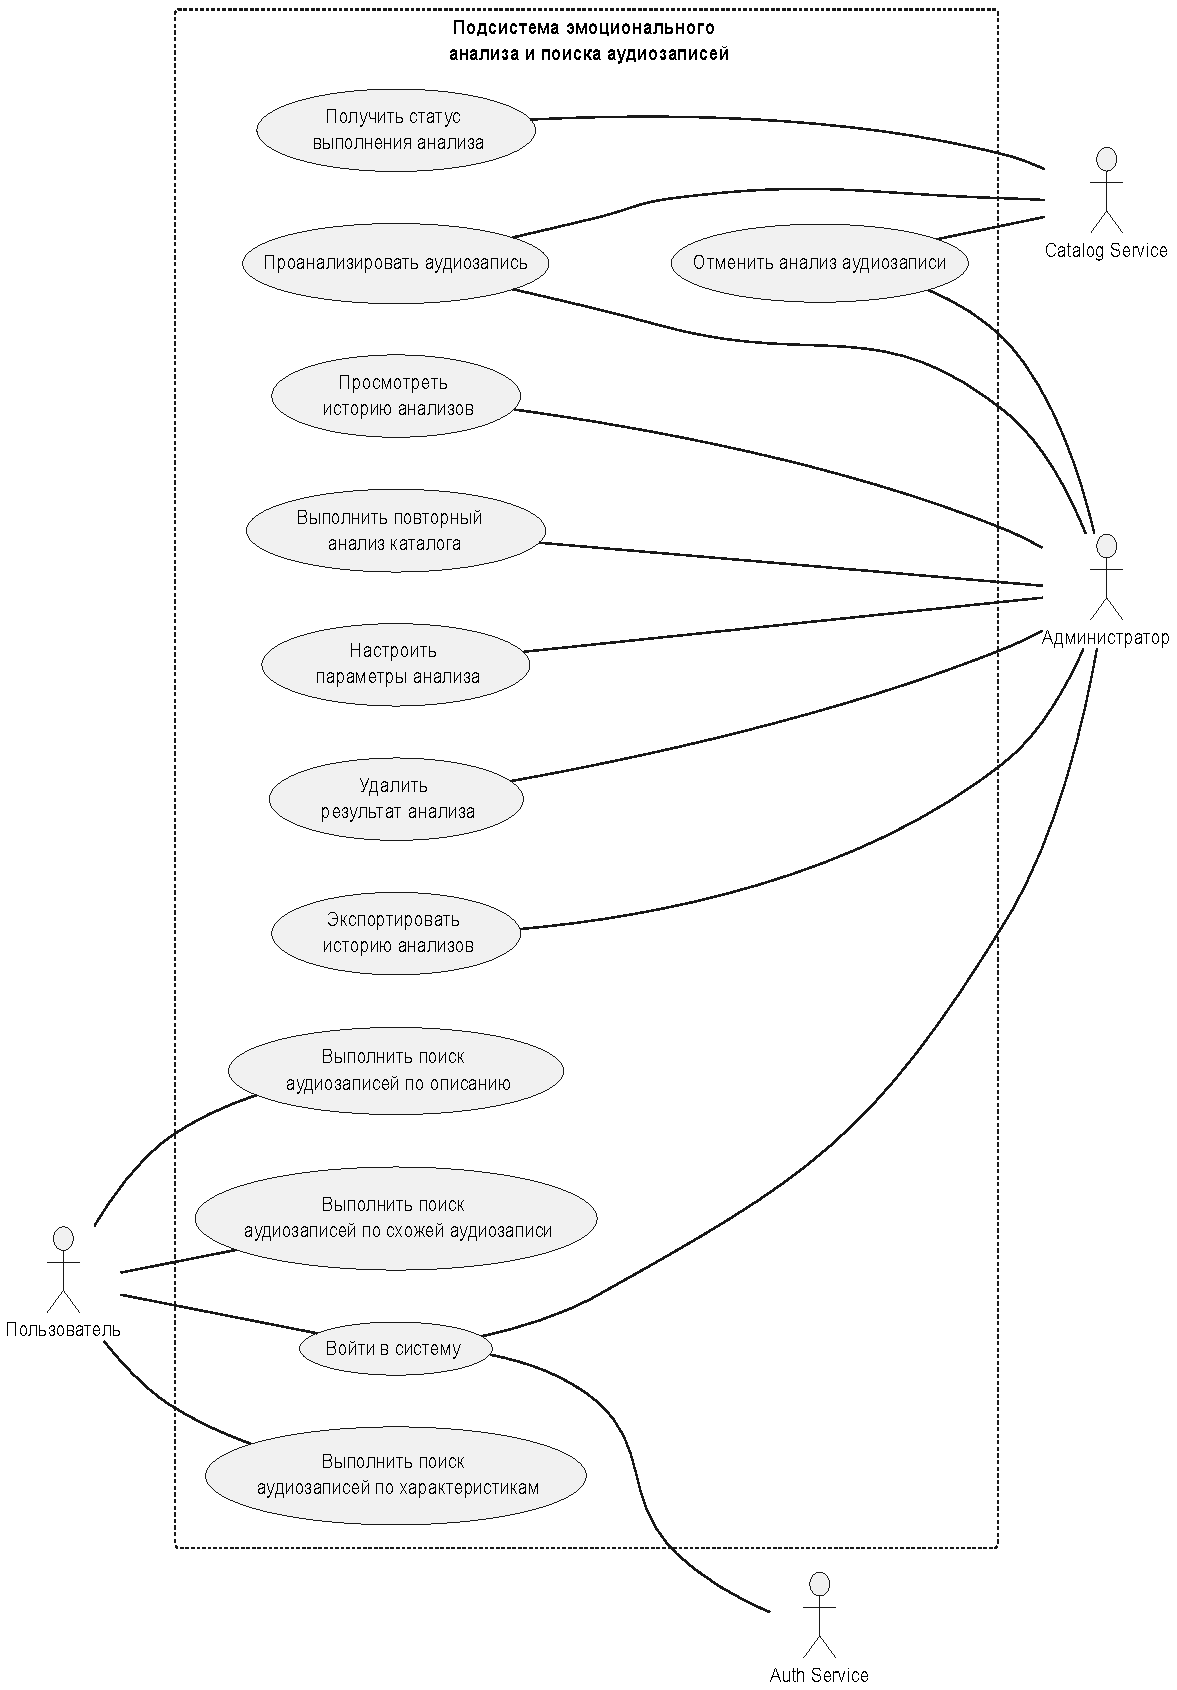
\includegraphics{figures/diagrams/initial-use-cases.pdf}}
 \caption{Исходная диаграмма прецедентов}\label{fig:uc-initial}
\end{figure}
На уточнённой диаграмме (рисунок~\ref{fig:uc-refined}) настройка параметров
включает выбор модели, её версии и порогов. Варианты просмотра истории
и экспорта показаны отношениями \texttt{extend}. В исходной модели три
варианта поиска связаны с общим прецедентом отношениями \texttt{include}.
При дальнейшем уточнении модели эти связи следует пересмотреть: выбор одного
из альтернативных способов поиска не означает обязательное выполнение всех
трёх.
\begin{figure}[H]
 \centering\adjustbox{max width=\textwidth,max height=0.73\textheight}{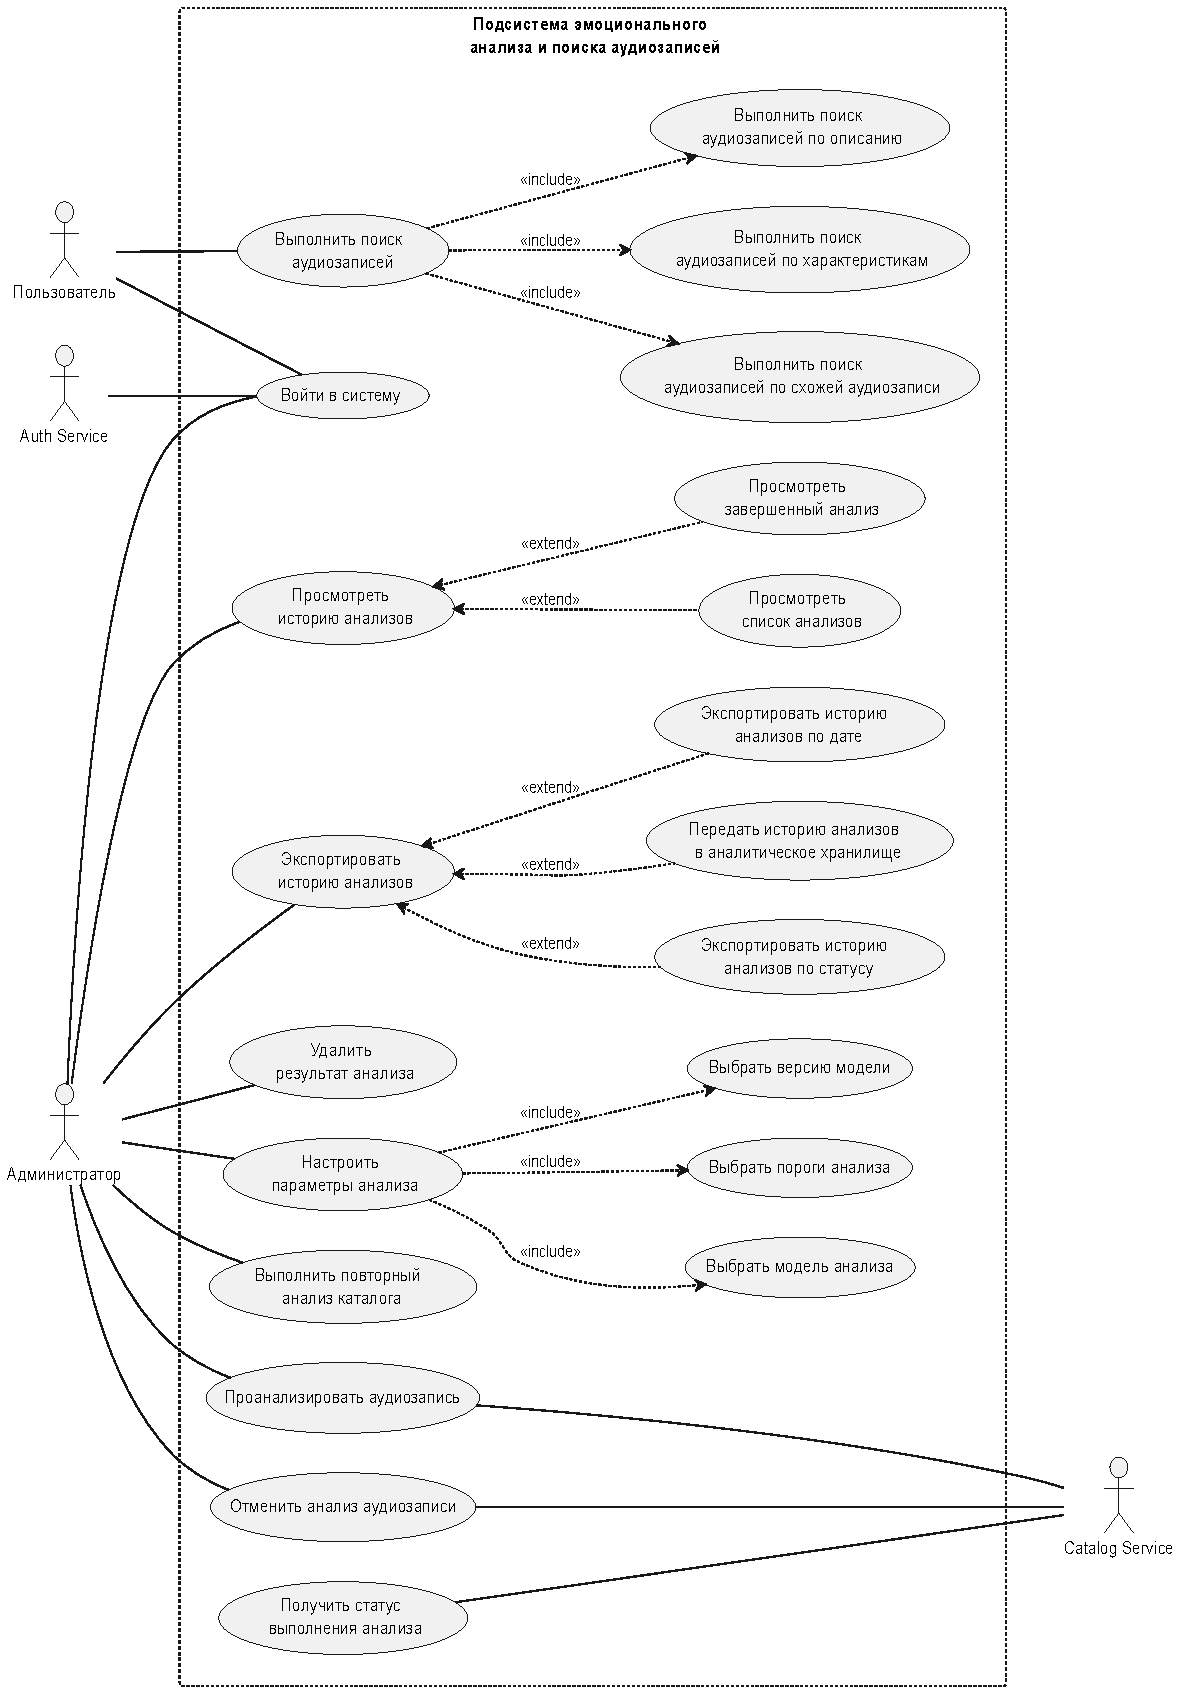
\includegraphics{figures/diagrams/clarified-use-cases.pdf}}
 \caption{Уточнённая диаграмма прецедентов}\label{fig:uc-refined}
\end{figure}

\subsection{Спецификации прецедентов}

Спецификации анализа аудиозаписи и поиска по описанию приведены в исходных
таблицах проекта [2].
\begingroup
\small
\setlength{\tabcolsep}{4pt}
\renewcommand{\arraystretch}{1.12}
\begin{longtable}{|L{0.23\textwidth}|L{0.65\textwidth}|}
\caption{Спецификация прецедента «Проанализировать аудиозапись»}\label{tab:spec-analysis}\\
\hline
\textbf{Раздел} & \textbf{Описание} \\
\hline
\endfirsthead
\multicolumn{2}{c}{Продолжение таблицы~\thetable}\\
\hline
\textbf{Раздел} & \textbf{Описание} \\
\hline
\endhead
Прецедент & Проанализировать аудиозапись \\
\hline
Краткое описание & Определение музыкальных и эмоциональных характеристик аудиозаписей, отбор оценок по порогам уверенности и сохранение результата для поиска и истории анализов. \\
\hline
Главные акторы & Администратор, Catalog Service. \\
\hline
Второстепенные акторы & Нет. \\
\hline
Предусловие & Администратор авторизован и имеет права на запуск анализа либо запрос поступает от Catalog Service, которому разрешён запуск анализа. \\
\hline
Основной поток & 1. Актор выбирает анализ всего каталога или одной либо нескольких аудиозаписей.\newline 2. Подсистема получает доступ к выбранным аудиофайлам.\newline 3. Подсистема проверяет доступность, целостность и поддерживаемый формат файлов.\newline 4. Подсистема проверяет наличие музыкальных характеристик в метаданных. Отсутствующие характеристики определяются при анализе.\newline 5. Параллельно подсистема определяет эмоциональные характеристики аудиозаписей.\newline 6. Подсистема отбирает оценки по соответствующим порогам уверенности.\newline 7. Подсистема обновляет характеристики аудиозаписей для поиска, используя принятые оценки и данные из метаданных.\newline 8. Подсистема сохраняет результат анализа.\newline 9. Подсистема предоставляет результат актору. \\
\hline
Постусловия & Результат анализа сохранён. Принятые оценки использованы для обновления характеристик аудиозаписей для поиска. Результат доступен инициатору и сохранён в истории анализов. \\
\hline
Альтернативные потоки & \textbf{E-1:} аудиофайл недоступен, повреждён или имеет неподдерживаемый формат. Подсистема сообщает инициатору об ошибке, анализ выбранных файлов не выполняется.\newline\newline \textbf{E-2:} нет оценок, прошедших пороги уверенности. Подсистема сохраняет результат анализа без таких оценок и оставляет характеристики для поиска без изменений.\newline\newline \textbf{E-3:} для аудиозаписи не хватает музыкальных характеристик в метаданных. Подсистема определяет отсутствующие характеристики и продолжает основной поток. \\
\hline
\end{longtable}
\endgroup

\begingroup
\small
\setlength{\tabcolsep}{4pt}
\renewcommand{\arraystretch}{1.12}
\begin{longtable}{|L{0.23\textwidth}|L{0.65\textwidth}|}
\caption{Спецификация прецедента «Поиск по естественно-языковому описанию»}\label{tab:spec-search}\\
\hline
\textbf{Раздел} & \textbf{Описание} \\
\hline
\endfirsthead
\multicolumn{2}{c}{Продолжение таблицы~\thetable}\\
\hline
\textbf{Раздел} & \textbf{Описание} \\
\hline
\endhead
Прецедент & Выполнить поиск аудиозаписей по естественно-языковому описанию \\
\hline
Краткое описание & Поиск аудиозаписей по текстовому описанию и дополнительным фильтрам с использованием семантического поиска по индексу. \\
\hline
Главные акторы & Пользователь. \\
\hline
Второстепенные акторы & Нет. \\
\hline
Предусловие & 1. Пользователь авторизован и имеет право выполнять поиск аудиозаписей.\newline 2. В поисковом индексе имеются данные об аудиозаписях. \\
\hline
Основной поток & 1. Пользователь вводит описание желаемой аудиозаписи.\newline 2. Пользователь при необходимости задаёт дополнительные фильтры по характеристикам аудиозаписей.\newline 3. Подсистема проверяет корректность описания и значений фильтров.\newline 4. Подсистема формирует векторное представление описания.\newline 5. Подсистема ищет аудиозаписи в поисковом индексе с учётом описания и фильтров.\newline 6. Подсистема упорядочивает найденные аудиозаписи по релевантности и предоставляет результаты пользователю. \\
\hline
Постусловия & 1. Пользователю предоставлен список подходящих аудиозаписей, упорядоченный по релевантности, либо сообщение об отсутствии результатов.\newline 2. Данные аудиозаписей и поискового индекса не изменены. \\
\hline
Альтернативные потоки & \textbf{E-1:} в описании или фильтрах есть ошибки. Подсистема сообщает пользователю об ошибке, поиск не выполняется.\newline\newline \textbf{E-2:} подходящие аудиозаписи не найдены. Подсистема сообщает пользователю об отсутствии результатов. \\
\hline
\end{longtable}
\endgroup


\subsection{Диаграммы деятельности}

Диаграмма анализа (рисунок~\ref{fig:activity-analysis}) отражает выбор
записей, проверку файлов, параллельное определение характеристик,
отбор оценок и сохранение результата. Ветвь ошибки завершается после
сообщения инициатору.
\begin{figure}[H]
 \centering\adjustbox{max width=\textwidth,max height=0.74\textheight}{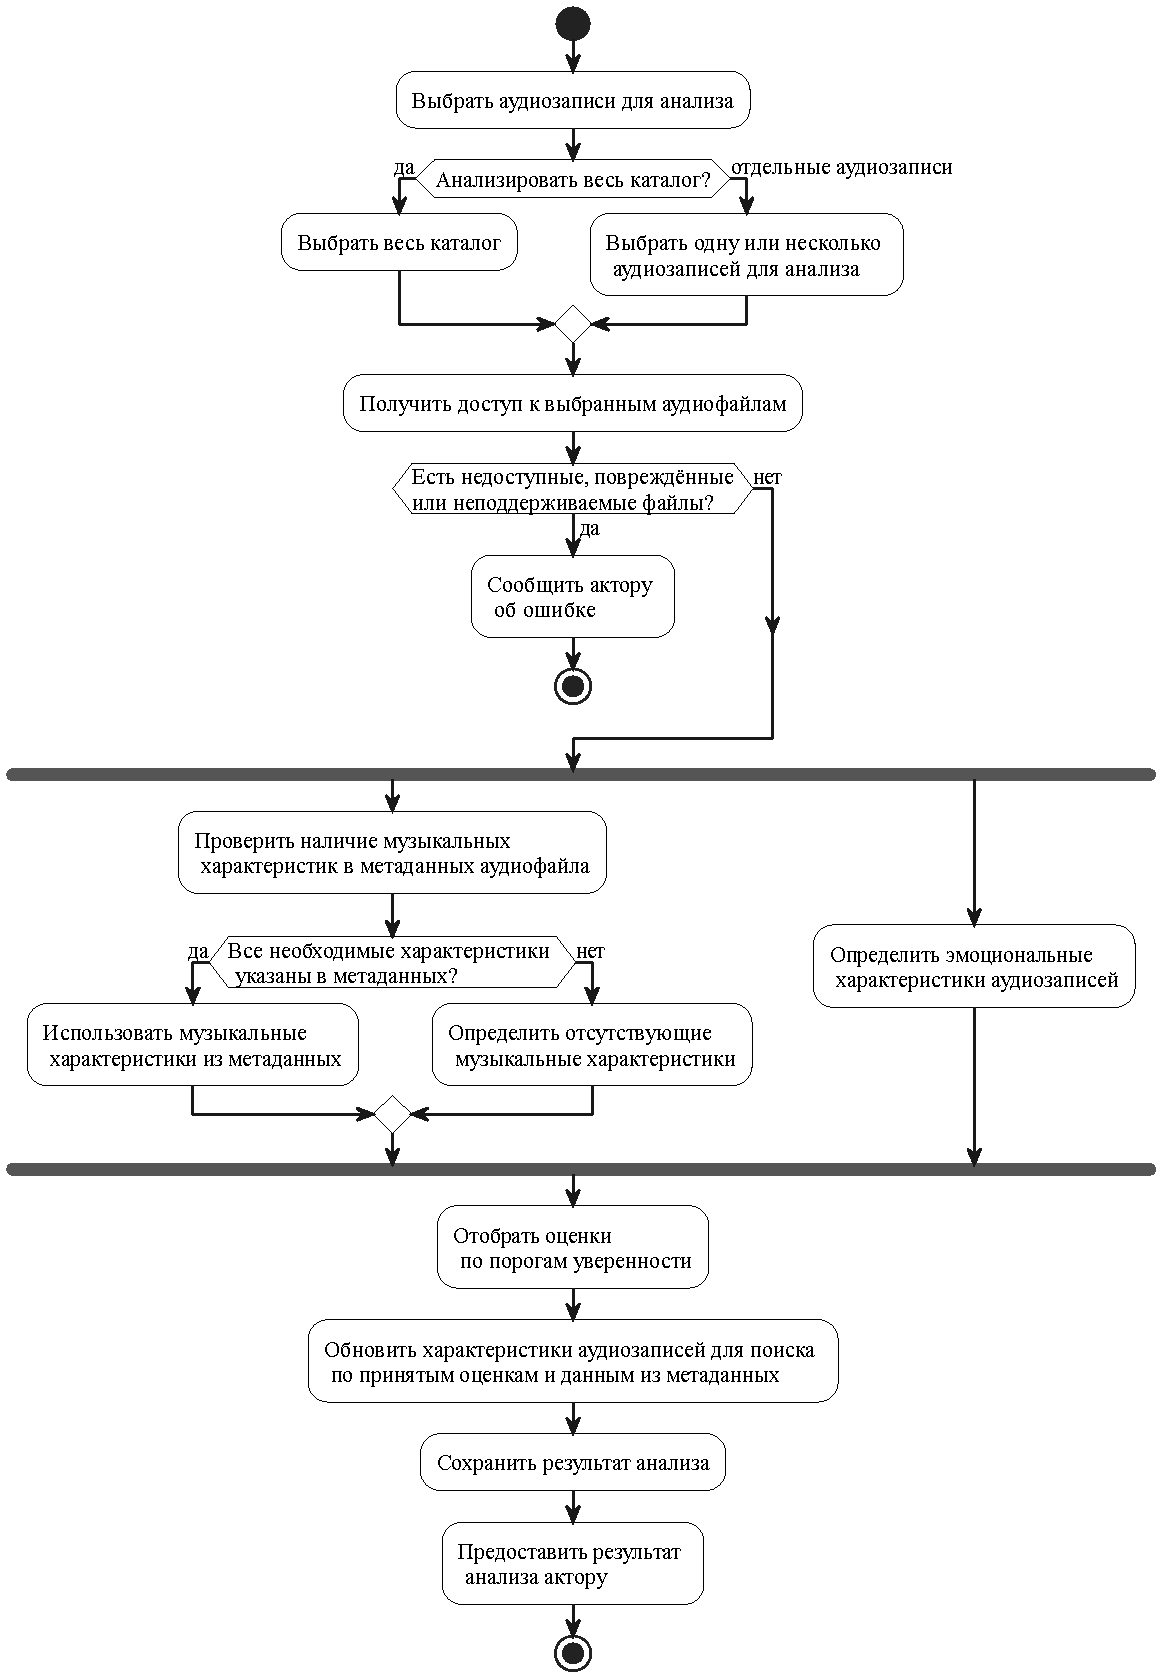
\includegraphics{figures/diagrams/analyze-audio-activity.pdf}}
 \caption{Диаграмма деятельности анализа аудиозаписи}\label{fig:activity-analysis}
\end{figure}

Диаграмма поиска (рисунок~\ref{fig:activity-search}) показывает ввод
описания, необязательные фильтры, проверку запроса, поиск в индексе
и выдачу результата. Отдельные ветви предусмотрены для ошибки ввода
и отсутствия подходящих записей.
\begin{figure}[H]
 \centering\adjustbox{max width=\textwidth,max height=0.74\textheight}{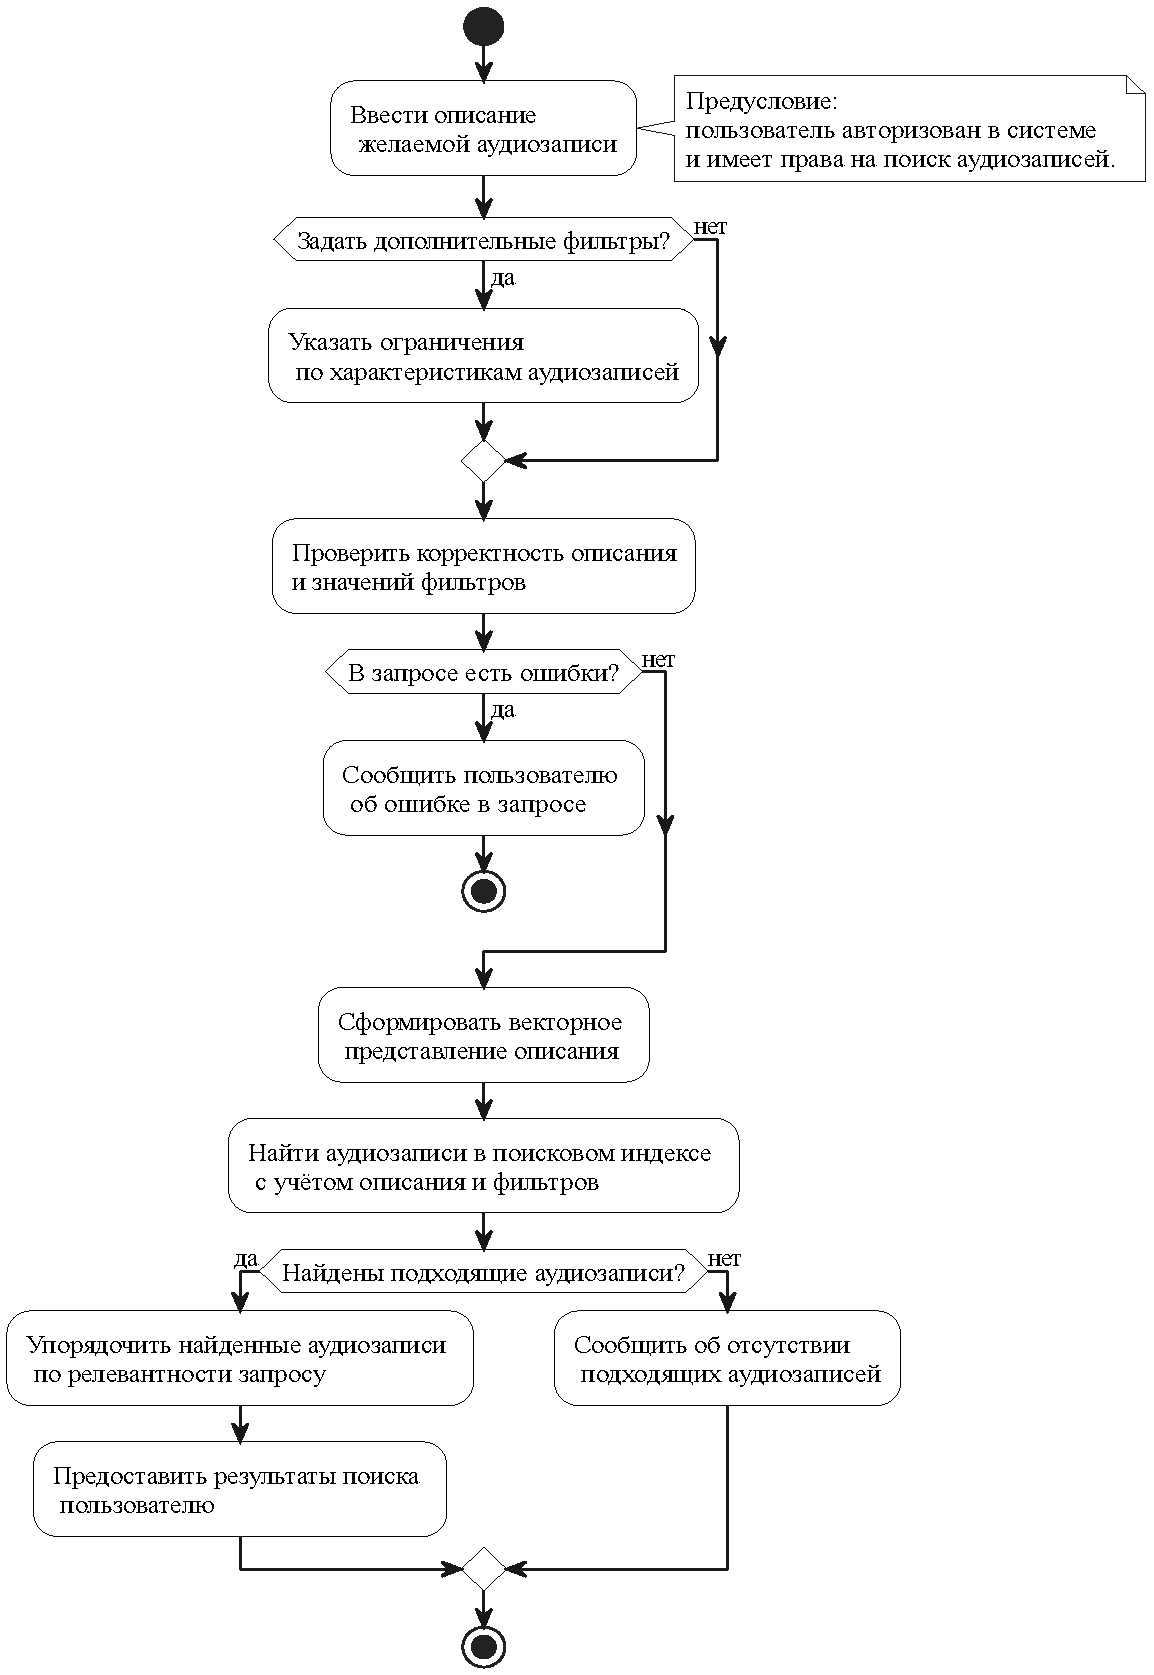
\includegraphics{figures/diagrams/search-audio-by-description-activity.pdf}}
 \caption{Диаграмма деятельности поиска по описанию}\label{fig:activity-search}
\end{figure}

\subsection{Диаграмма классов предметной области}

Развёрнутая диаграмма классов (рисунок~\ref{fig:classes}) содержит
аудиозапись, пользователя и роль, задание анализа, модель, профили весов
и порогов, а также оценки уверенности. Задание связано с аудиозаписью и профилями;
оценки принадлежат заданию и могут относиться к тегу или эмоциональной метке.
\begin{figure}[H]
 \addtocounter{figure}{1}
 \centering\adjustbox{max width=\textwidth,max height=0.75\textheight}{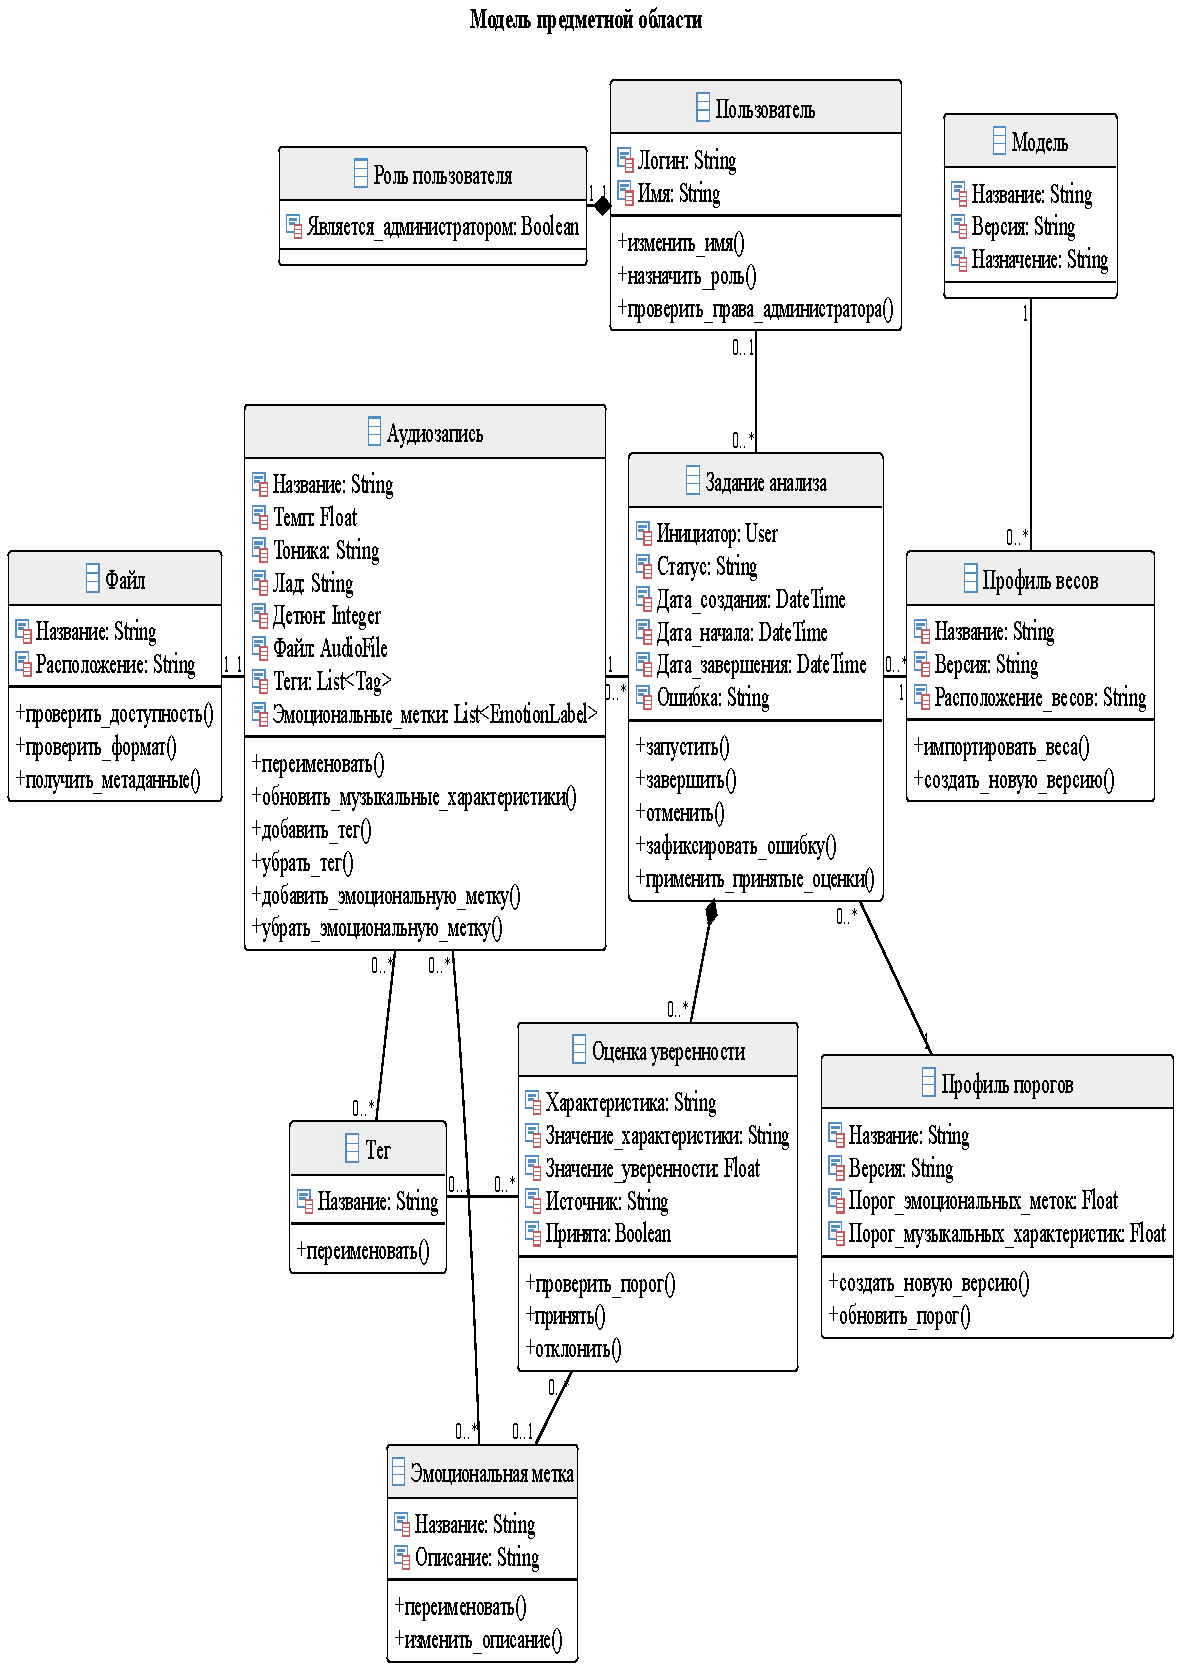
\includegraphics{figures/diagrams/classes-diagram.pdf}}
 \caption{Развёрнутая диаграмма классов предметной области}\label{fig:classes}
\end{figure}

\subsection{Прототип пользовательского интерфейса}

Прототипы показывают страницы администратора для запуска анализа, контроля
заданий, просмотра истории и настройки модели. Аудиофайлы и метаданные
поступают из каталога; на страницах отображаются действия администратора
и состояние обработки.

На экране анализа доступен каталог с поиском, фильтрами и запуском обработки
отдельной записи или выбранной группы (рисунки~\ref{fig:proto1} и~\ref{fig:proto2}).
\begin{figure}[H]\centering
 \reportScreenshot{figures/01-analyze-audio.png}
 \caption{Каталог записей для запуска анализа}\label{fig:proto1}
\end{figure}
\begin{figure}[H]\centering
 \reportScreenshot{figures/02-analyze-audio.png}
 \caption{Выбор аудиозаписей для анализа}\label{fig:proto2}
\end{figure}

Состояние выполняемых заданий и сведения о конкретном запуске показаны
на рисунках~\ref{fig:proto3} и~\ref{fig:proto4}.
\begin{figure}[H]\centering
 \reportScreenshot{figures/03-analyze-audio-active-task.png}
 \caption{Список активных заданий анализа}\label{fig:proto3}
\end{figure}
\begin{figure}[H]\centering
 \reportScreenshot{figures/04-analyze-audio-active-task-detailed.jpg}
 \caption{Подробные сведения об активном задании}\label{fig:proto4}
\end{figure}

Для повторной обработки всего каталога предусмотрен отдельный сценарий
(рисунок~\ref{fig:proto5}). История запусков содержит статусы и сведения
о качестве результатов, а также предоставляет экспорт (рисунки~\ref{fig:proto6}
и~\ref{fig:proto7}).
\begin{figure}[H]\centering
 \reportScreenshot{figures/05-analyze-catalog.png}
 \caption{Запуск анализа каталога}\label{fig:proto5}
\end{figure}
\begin{figure}[H]\centering
 \reportScreenshot{figures/06-view-analisis-history.png}
 \caption{Просмотр истории анализов}\label{fig:proto6}
\end{figure}
\begin{figure}[H]\centering
 \reportScreenshot{figures/07-export-analysis-history.png}
 \caption{Экспорт истории анализов}\label{fig:proto7}
\end{figure}

Вход администратора показан на рисунке~\ref{fig:proto8}. Операция удаления
результата представлена последовательностью выбора, подтверждения и уведомления
(рисунки~\ref{fig:proto9}-\ref{fig:proto11}).
\begin{figure}[H]\centering
 \reportScreenshot{figures/08-admin-login.png}
 \caption{Вход администратора}\label{fig:proto8}
\end{figure}
\begin{figure}[H]\centering
 \reportScreenshot{figures/09-delete-analisis-result.png}
 \caption{Выбор результата для удаления}\label{fig:proto9}
\end{figure}
\begin{figure}[H]\centering
 \reportScreenshot{figures/10-delete-analisis-result.png}
 \caption{Подтверждение удаления результата}\label{fig:proto10}
\end{figure}
\begin{figure}[H]\centering
 \reportScreenshot{figures/11-delete-analisis-result-notifications.png}
 \caption{Уведомление об удалении результата}\label{fig:proto11}
\end{figure}

Результаты анализа и характеристики записи представлены на
рисунках~\ref{fig:proto12} и~\ref{fig:proto13}. Экран параметров модели
позволяет задать версию модели и пороги уверенности (рисунок~\ref{fig:proto14});
отмена задания показана на рисунке~\ref{fig:proto15}.
\begin{figure}[H]\centering
 \reportScreenshot{figures/12-view-result-of-analysis.png}
 \caption{Просмотр результата анализа}\label{fig:proto12}
\end{figure}
\begin{figure}[H]\centering
 \reportScreenshot{figures/13-view-result-of-analysis.png}
 \caption{Подробные характеристики результата анализа}\label{fig:proto13}
\end{figure}
\begin{figure}[H]\centering
 \reportScreenshot{figures/14-config-model-parameters.png}
 \caption{Настройка параметров модели и порогов}\label{fig:proto14}
\end{figure}
\begin{figure}[H]\centering
 \reportScreenshot{figures/15-cancel-analyze-task.png}
 \caption{Отмена задания анализа}\label{fig:proto15}
\end{figure}

